\setlength{\baselineskip}{20pt}
\chapter{基于稀疏学习和梯度扰动的梯度泄露防护}
\label{cha:chap4}

上一章提出了一个联邦学习系统,旨在保护车联网中的数据隐私。然而,本文的关注点不仅仅在于联邦学习的应用,更着重于联邦学习本身。现有研究表明,原始的联邦学习并非绝对安全,攻击者可以根据泄露的梯度数据推导出原始的训练数据。因此,本章将进一步研究保护数据隐私的方法,以防止敌手从共享的梯度中重构出敏感的训练样本。为此,本章提出了一个基于稀疏学习和梯度扰动的梯度泄露防护方案。该方案的核心思想分为两部分。首先,利用系数学习方法将训练数据表示为稀疏字典学习(DL)的形式,从而降低数据的可识别性。其次,为了进一步增强模型的鲁棒性,对全连接(FC)层的梯度进行了随机扰动,以抵抗梯度泄露的攻击。最后,本章在不同的数据集和攻击场景下进行了实验,最终验证了所提出方法的有效性和优越性。这种防御方法可以与现有的联邦学习系统结合,而无需修改训练协议。通过广泛的实验,还证明了所提出的方法可以有效地抵抗重构攻击,同时具有高效性和可忽略的性能损失。

\section{相关工作和技术介绍}

\subsection{特征提取与稀疏学习}

在机器学习中,数据的属性通常称为“特征”(feature),与当前学习任务有关的属性称为“相关特征”(relevant feature),与当前学习任务无关的属性称为“无关特征" (irrelevant feature)。从给定的特征集合中选择出一个相关特征的子集,这个过程称为 “特征选择"(feature selection)。特征选择是“数据预处理”(data preprocessing)的一个重要步骤,在实际的机器学习任务中,通常需要先对数据进行特征选择,然后再用选出的特征来训练学习器。特征选择的目的有两个:一是为了缓解“维数灾难”(curse of dimensionality)问题,这是由于特征过多导致的。如果能够从众多的特征中挑选出最重要的特征,那么后续的学习过程就可以只在这些特征上建立模型,从而降低维度,减少计算和存储的开销,提高模型的可解释性。二是为了降低学习任务的难度,因为去除无关特征可以消除数据中的噪声和冗余,提高数据的质量,从而提高学习器的性能。特征选择过程要注意不要丢失重要特征,否则会导致信息的损失,影响学习器的泛化能力。有些特征虽然包含的信息可以从其他特征中推导出来,但是它们并不是无用的,这些特征称为“冗余特征"(redundant feature)。冗余特征在某些情况下是有益的,比如当它们恰好对应了学习任务所需的“中间概念”时,它们可以降低学习任务的难度。特征选择方法通常由两个部分组成:特征子集的搜索机制和特征子集的评价机制。根据这两个部分的不同,特征选择方法可以分为三类:过滤式(filter)、包裹式(wrapper)和嵌入式(embedding)。

把数据集$D$看作一个矩阵,其中每一行代表一个样本,每一列代表一个特征。特征选择要解决的问题是特征的“稀疏性”,即矩阵中的许多列与当前的学习任务无关,如果能够通过特征选择去掉这些列,那么学习器的训练过程就只需要在一个较小的矩阵上进行,这样可以降低学习任务的难度,减少计算和存储的开销,提高模型的可解释性。另一种稀疏性是指矩阵中存在很多零元素,但这些零元素并不是以整列或整行的形式出现的,而是分散在矩阵中的不同位置。这种稀疏性对学习任务来说是有利的,比如线性支持向量机在文本数据上的表现就很好,这是因为文本数据在使用字频表示后具有很高的稀疏性,使得大多数问题变得线性可分。同时,这种稀疏性也不会造成存储上的负担,因为稀疏矩阵有很多高效的存储方法。

“字典学习”(dictionary learning)或者“稀疏编码”(sparse coding)则是其中一种将样本转换为字典中的线性组合的方法,它们能够赋予密集表示的样本稀疏性,从而简化学习任务,降低模型的复杂度。给定数据集$\boldsymbol{x}_1, \boldsymbol{x}_2, \ldots, \boldsymbol{x}_m$,字典学习的最简单形式可以表示为以下优化问题:
\begin{equation}
\min_{\mathbf{B},\boldsymbol{\omega}_i}\sum_{i=1}^m\|\boldsymbol{x}_i-\mathbf{B}\boldsymbol{\omega}_i\|_2^2+\lambda\sum_{i=1}^m\|\boldsymbol{\omega}_i\|_1\:,
\label{eq:dictionary_learning}
\end{equation}
其中$\mathbf{B} \in \mathbb{R}^{d \times k}$是字典矩阵,$k$是字典的词汇量,通常由用户指定。$\boldsymbol{\omega}_i \in \mathbb{R}^k$表示样本$\boldsymbol{x}_i \in \mathbb{R}^d$的稀疏表示。式\ref{eq:dictionary_learning}中的第一项旨在使$\boldsymbol{\omega}_i$能够尽可能地重构$\boldsymbol{x}_i$,而第二项则旨在使$\boldsymbol{\omega}_i$尽可能地稀疏。

为了求解式\ref{eq:dictionary_learning},可以采用变量交替优化的策略。首先,固定字典$\mathbf{B}$,优化$\boldsymbol{\omega}_i$。这时,可以将式\ref{eq:dictionary_learning}按分量展开,发现其中没有涉及到$\omega_i^u \omega_i^v$($u \neq v$)这样的交叉项。因此,可以参考LASSO的解法,求解以下问题,从而得到每个样本$\boldsymbol{x}_i$的稀疏表示$\boldsymbol{\omega}_i$:

\begin{equation}
\min_{\boldsymbol{\omega}_i}\|\boldsymbol{x}_i-\mathbf{B}\omega_i\|_2^2+\lambda\|\boldsymbol{\omega}_i\|_1\:.
\label{eq:dictionary_learning_3}
\end{equation}

接下来,固定$\boldsymbol{\omega}_i$,优化字典$\mathbf{B}$。这时,可以将式\ref{eq:dictionary_learning}写为以下形式:

\begin{equation}
\min_{\mathbf{B}}\|\mathbf{X}-\mathbf{BA}\|_{F}^{2},
\label{eq:dictionary_learning_4}
\end{equation}

其中$\mathbf{X} = (\boldsymbol{x}_1, \boldsymbol{x}_2, \ldots, \boldsymbol{x}_m) \in \mathbb{R}^{d \times m}$,$\mathbf{A} = (\boldsymbol{\omega}_1, \boldsymbol{\omega}_2, \ldots, \boldsymbol{\omega}_m) \in \mathbb{R}^{k \times m}$,$\|\cdot\|_F$表示矩阵的Frobenius范数。式\ref{eq:dictionary_learning_4}有多种求解方法,其中一种常用的方法是基于逐列更新策略的KSVD。令$b_i$表示字典矩阵$B$的第$i$列,$\omega_i$表示稀疏矩阵$A$的第$i$行,式\ref{eq:dictionary_learning_4}可重写为:

\begin{equation}\begin{aligned}
\operatorname*{min}_{\mathbf{B}}\|\mathbf{X}-\mathbf{BA}\|_{F}^{2}& =\min_{\boldsymbol{b}_{i}}\left\|\mathbf{X}-\sum_{j=1}^{k}\boldsymbol{b}_{j}\boldsymbol{\omega}^{j}\right\|_{F}^{2}  \\
&=\min_{\boldsymbol{b}_i}\left\|\left(\mathbf{X}-\sum_{j\neq i}\boldsymbol{b}_j\boldsymbol{\omega}^j\right)-\boldsymbol{b}_i\boldsymbol{\omega}^i\right\|_F^2 \\
&=\min_{\boldsymbol{b}_{i}}\left\|\mathbf{E}_{i}-\boldsymbol{b}_{i}\boldsymbol{\omega}^{i}\right\|_{F}^{2}\:.
\end{aligned}
\label{eq:dictionay_learning 4}
\end{equation}

在更新字典的第$i$列时,其他各列都保持固定。因此,有$\mathbf{E}_i=\sum_{j\neq i}\boldsymbol{b}_j\boldsymbol{\omega}^j$是一个固定项。为避免直接对$\mathbf{E}_i$进行奇异值分解而破坏稀疏性,KSVD算法对$\mathbf{E}_i$和$\omega_i$进行特殊处理:$\omega_i$仅保留非零元素,$\mathbf{E}_i$则仅保留与$\boldsymbol{b}_i$和$\boldsymbol{\omega}^i$的非零元素相乘的项,然后再进行奇异值分解,以保持第一步得到的稀疏性。通过对字典矩阵$B$进行初始化,然后反复迭代上述两步,最终就可以得到字典$B$和样本$x_i$的稀疏表示$\omega_i$。在字典学习的过程中,用户可以通过设置字典的词汇量$k$来控制字典的规模,从而影响稀疏表示的程度。

% 有时间把K-SVD扩充一下:https://blog.csdn.net/qq_37085158/article/details/122559053 https://ieeexplore.ieee.org/document/1710377

\subsection{差分隐私}

如图\ref{fig:three major privacy guarantees}所示,数据隐私技术涵盖了多个方面,包括模糊技术、扰动技术、加密技术、混合隐私技术、分布式计算框架和区块链技术。其中,扰动技术专注于对数据本身进行扰动,主要体现在差分隐私技术上。差分隐私通过在数据上直接添加随机噪声,或者将原始值以一定概率扰动为随机值,从而实现隐私保护。与传统的统计披露限制方法(如k-匿名)不同,差分隐私能够抵御具有任意背景知识和计算能力的攻击,并最大限度地延缓因多次发布而造成的隐私泄露风险。此外,差分隐私不依赖算法和参数的保密性,且任何计算都无法削弱已有的隐私保障。由于严格的数学保证和良好的隐私性质,差分隐私已被谷歌、苹果、微软、脸书、领英及美国人口普查局等机构采纳,并在生产系统中用于保护参与者的隐私。

\begin{figure}[htb]
\centering
    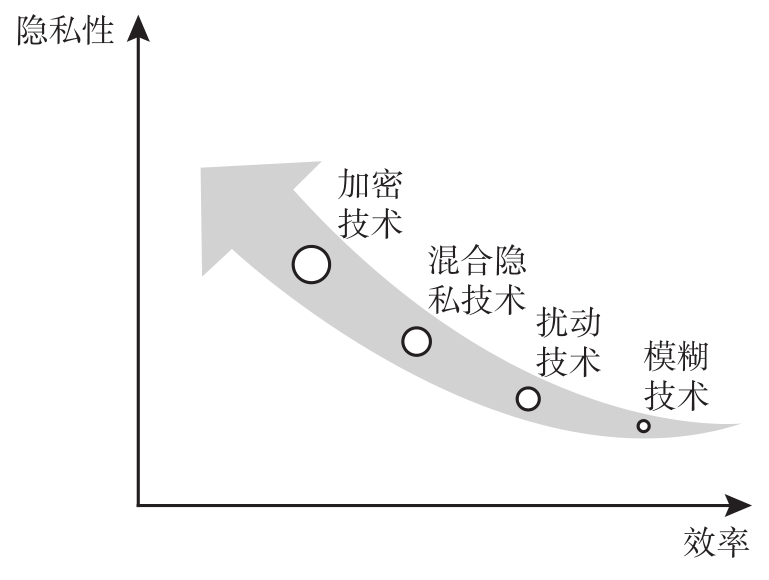
\includegraphics[scale=1.5]{figures/chapter4/Comparison of privacy and efficiency of different privacy technologies.jpg}
    % \caption{FL-vgg16 Confusion Matrix}
    \caption{不同隐私技术在隐私性与效率上的对比}
    \label{fig:three major privacy guarantees}
\end{figure}

然而,通过扰动保护数据隐私会导致数据可用性降低,从而影响计算结果的准确性。因此,在保护数据隐私的前提下,如何尽可能提高扰动对数据可用性的影响,成为该技术的核心问题。通常,满足差分隐私的算法有两种数据扰动方式:一种是直接在计算结果上添加噪声,常用的包括拉普拉斯机制、指数机制等;另一种是以一定的概率对数据进行扰动,即随机响应机制。在定义差分隐私之前,首先定义两个数据库之间的距离。

数据库距离定义。将数据库$x$的$L_1$范数记作$\parallel x\parallel_1=\sum_{i=1}^{| x|}\parallel x\parallel_i$,则两个数据库之间的$L_1$距离便是$\parallel x-y\parallel_1$。若将$\parallel x\parallel_1$作为数据库$x$大小的度量,即$x$中一共包含几行记录,则$\parallel x-y\parallel_1$便用于度量数据库$x$和$y$中有几行不同的记录,也就是数据库之间的距离。

差分隐私定义。对于一个随机算法$\mathcal{M}$,其值域为$Range(\mathcal{M})$,如果对$Range(\mathcal{M})$的任意子集$S$和$\mathcal{M}$定义域上的一对相邻数据集$x$和$y$($\parallel x - y \parallel_1 \le 1$),有$\Pr[\mathcal{M}(x)\in S]\leq e^{\varepsilon}Pr[\mathcal{M}(y)\in S]+\delta$,则称算法$M$满足$(\varepsilon ,\delta)$-差分隐私。其中,$\Pr[\mathcal{M}(x)\in S]$表示在输入为$x$时,机制$\mathcal{M}$的输出落在集合$S$中的概率。这里,$\mathcal{M}$是一个隐私保护机制,例如一个加噪声的查询回答器。$\Pr[\mathcal{M}(y)\in S]$表示输入为$y$时,同样的机制$\mathcal{M}$的输出落在集合$S$中的概率。注意,$x$和$y$是相邻的输入,即它们在数据上非常接近。$e^{\varepsilon}$是一个指数项,用于衡量输入$x$和$y$之间的相似性,表示在隐私保护机制中,输出在$x$和$y$之间的概率差异。$\delta$是一个小常数(通常接近零),表示额外的隐私参数,当$\delta=0$时,则说算法$M$满足$\varepsilon $-差分隐私。这个不等式表明:如果一个机制$\mathcal{M}$是差分隐私的,那么在输入$x$和$y$之间的输出概率不会有显著的差异。也就是说,$\mathcal{M}$确保了相似输入的输出概率“接近”,同时允许一小部分额外的隐私损失(由$\delta$控制)。可以看到,当$\varepsilon $越小意味着,攻击者越难区分这对相邻数据集,保护程度越高。反之,当$\varepsilon $越大时,保护程度就越低。一般情况下,也把$\varepsilon $叫作隐私预算。

\begin{figure}[htb]
\centering
    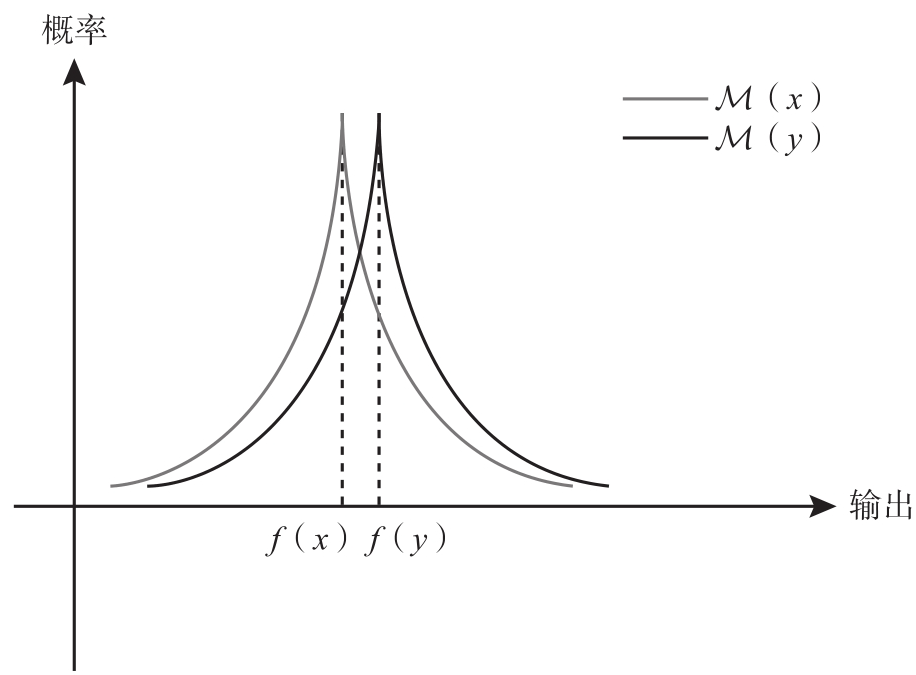
\includegraphics[scale=1]{figures/chapter4/dp figure.png}
    % \caption{FL-vgg16 Confusion Matrix}
    \caption{差分隐私算法在邻近数据集上的输出概率}
    \label{fig:dp figure}
\end{figure}

函数敏感度。对于一个查询函数$f(·)$,它作用于一对相邻数据集$x$和$x′$,返回结果的最大变化范围,便是该查询函数的函数敏感度:
\begin{equation}\mathrm{Sensitivity}(f)=\max_{x,x^{\prime}}\parallel f(x)-f(x^{\prime})\parallel_{1}
\end{equation}
需要注意的是,函数敏感度只由查询函数本身决定,与查询的数据集无关。

拉普拉斯差分隐私。对于连续型数据的查询结果,拉普拉斯机制在查询结果上加入一个满足分布$\text{Lap}\bigg(0,\frac{\text{Sensitivity}(f)^{\odot}}{\varepsilon}\bigg)$的噪声,来实现差分隐私。其中$Sensitivity(f)$为查询函数敏感度,$\varepsilon$为隐私预算。以$x$表示被查询的数据库,$M(x)$表示最后的查询结果,$f(x)$表示原先查询函数返回的查询结果,$Y$表示满足拉普拉斯分布的噪声,即$Y\thicksim\text{Lap}\bigg(0,\frac{\text{Sensitivity}(f)}{\varepsilon}\bigg)$,则拉普拉斯机制可以表示为$M(x)=f(x)+Y$。

拉普拉斯机制满足$\varepsilon$-差分隐私。根据这一定义,可以看到隐私预算越小、扰动越大,则结果的可用性越小,隐私保护程度越高。下面将证明拉普拉斯机制满足$\varepsilon $-差分隐私。假设$x$和$y$为两个相邻数据集,即$\parallel x - y \parallel_1 \le 1$,而$f$表示未加噪的查询函数返回的结果,$M(x)$表示最后查询函数返回的结果,$p_x$为$M(x)$的概率密度函数,$p_y$为$M(y)$的概率密度函数。比较位于$f$值域中的任意一点$z$,有

\begin{equation}
\begin{aligned}
\frac{p_x(z)}{p_y(z)} &= \prod_{i=1}^{k} \frac{\exp\left(\frac{e|f(x)_i - z_i|}{\Delta f}\right)}{\exp\left(\frac{e|f(y)_i - z_i|}{\Delta f}\right)} \\
&= \prod_{i=1}^{k} \exp\left(\frac{e(|f(y)_i - z_i| - |f(x)_i - z_i|)}{\Delta f}\right) \\
& \leq \prod_{i=1}^{k} \exp\left(\frac{e(|f(x)_i - f(y)_i|)}{\Delta f}\right) \\
&= \exp\left(\frac{e \cdot ||f(x) - f(y)||_1 }{ {\Delta f}}\right)
\leq \exp(e)
\end{aligned}
\end{equation}

上式第一个不等式可根据三角不等式得出,最后一个不等式则根据函数敏感度定义和$\parallel x - y \parallel_1 \le 1$得出。对称地,我们有[插图]。证毕。

差分隐私会不可避免地引入统计噪声。隐私保护需要随机性,不平凡(最少有两种不同输出)的确定算法无法满足差分隐私,如图8.3所示。对于不平凡的确定算法,一定存在两个仅相差一条记录的数据集(如红色和绿色的正方形)被同一函数映射到不同结果(如红色和绿色的三角形)的情况,这将使攻击者明确这条记录的存在或缺失,从而泄露应答者的隐私。尽管差分隐私算法具有相当大的灵活性,但不确定性的增加必然会造成统计效用的损失。一种简单的办法是不断提升样本容量,从而使差分隐私噪声所造成的误差远小于系统的固有误差(如抽样误差)。如何缓解统计隐私和效用的紧张关系是差分隐私研究的核心问题。

差分隐私不依赖算法和参数的保密性。柯克霍夫(Kerckhof)原则告诉我们,密码系统的安全不应依赖除密钥以外任何事物的保密性,这无疑与仰仗算法保密的模糊式安全(security by obscurity)形成了鲜明对比。在差分隐私之前,统计披露控制大多以黑箱形式进行。统计机构需要隐藏数据的变换程度,从而保留数据用户对分析结果的不确定性。差分隐私继承了Kerckhof原则,只有随机种子需要保密,而隐私算法和参数的公开并不影响其所提供的隐私保证。这种透明性首次将隐私与效用的权衡取舍置于众目之下,既能帮助政策制定者做出科学、合理的决策,也能强化人们对所用隐私技术的理解、信任与监督

\begin{figure}[htb]
\centering
    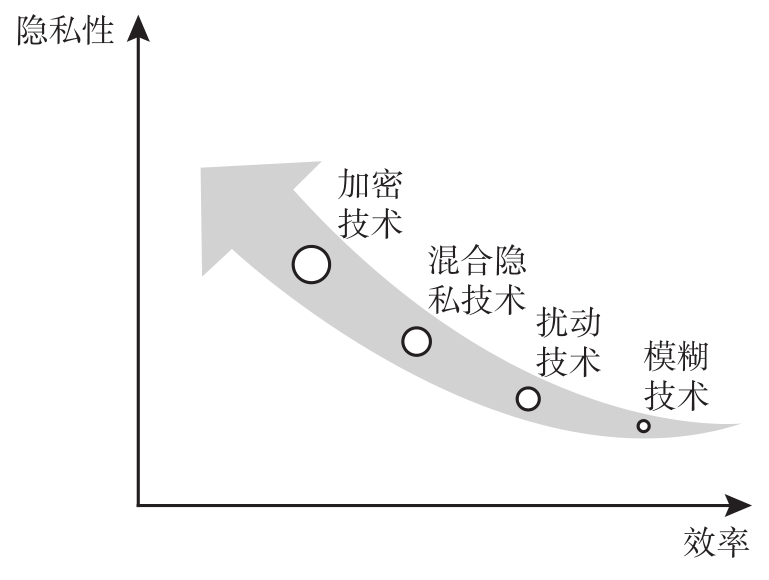
\includegraphics[scale=0.5]{figures/chapter4/Comparison of privacy and efficiency of different privacy technologies.jpg}
    % \caption{FL-vgg16 Confusion Matrix}
    \caption{不同隐私技术在隐私性与效率上的对比}
    \label{fig:Cluster the cars in the region}
\end{figure}

差分隐私用于隐私保护时,需要处理的数据可以分为两大类——连续型数据和离散型数据。连续型数据往往是一个连续区间内的数值取值,如树的高度、房屋的宽度等;离散型数据则可以对数据进行一一列举,如彩虹的七种颜色、人的五根手指等。差分隐私的主要思想是对数据添加扰动,而对于不同类型的数据,扰动的类型也不相同。对连续型数据,常用的扰动机制是拉普拉斯机制。对离散型数据,常用的是指数机制。拉普拉斯机制在介绍拉普拉斯机制前,需要先介绍一下敏感度。差分隐私通过对数据添加扰动(加噪)来保护用户隐私,如果扰动过大,则会导致数据可用性太差影响数据使用,如果扰动过小,则可能会导致用户隐私被攻击者获取、保护能力下降。由此可见,扰动的大小是差分隐私中一个重要的量,敏感度便是用于控制扰动大小的参数。定义4.3 函数敏感度.对于一个查询函数f(·),它作用于一对相邻数据集x和x′,返回结果的最大变化范围,便是该查询函数的函数敏感度

\begin{equation}
\mathrm{Sensitivity}(f)=\max_{x,x^{\prime}}\parallel f(x)-f(x^{\prime})\parallel_{1}
\end{equation}

需要注意的是,函数敏感度只由查询函数本身决定,与查询的数据集无关。有了函数敏感度的定义后,接下来介绍拉普拉斯机制。对于连续型数据的查询结果,拉普拉斯机制在查询结果上加入一个满足分布$\begin{aligned}\text{Lap}\bigg(0,&\frac{\text{Sensitivity}(f)^{\odot}}{\varepsilon}\bigg)\end{aligned}$的噪声,来实现差分隐私。其中Sensitivity(f)为查询函数敏感度,$\varepsilon$ 为隐私预算。

定义4.4 拉普拉斯机制.以$x$表示被查询的数据库,$M(x)$表示最后的查询结果,$f(x)$表示原先查询函数返回的查询结果,$Y$表示满足拉普拉斯分布的噪声,即$\begin{aligned}Y&\thicksim\text{Lap}\bigg(0,\frac{\text{Sensitivity}(f)}{\varepsilon}\bigg)\end{aligned}$,则拉普拉斯机制可以表示为$M(x)=f(x)+Y$

拉普拉斯机制满足$\varepsilon $-差分隐私。根据这一定义,可以看到隐私预算越小、扰动越大,则结果的可用性越小,隐私保护程度越高。下面将证明拉普拉斯机制满足$\varepsilon $-差分隐私。假设$x$和$y$为两个相邻数据集,即$\parallel x - y \parallel_1 \le 1$,而f表示未加噪的查询函数返回的结果,$M(x)$表示最后查询函数返回的结果,$p_x$为$M(x)$的概率密度函数,$p_y$为$M(y)$的概率密度函数。比较位于f值域中的任意一点z,有
\begin{equation}
\frac{p_x(z)}{p_y(z)}=\prod_{i=1}^k\left(\frac{\exp\left(-\frac{\boldsymbol{\varepsilon}\left|f(x)_i-z_i\right. |}{\Delta f}\right)}{\exp\left(-\frac{\boldsymbol{\varepsilon}\left|f(y)_i-z_i\right. |}{\Delta f}\right)}\right)
\end{equation}

上式第一个不等式可根据三角不等式得出,最后一个不等式则根据函数敏感度定义和$\parallel x - y \parallel_1 \le 1$得出。对称地,我们有[插图]。证毕。

\section{基于稀疏学习和梯度扰动的梯度泄露防护方案}

\begin{figure}[htb]
\centering
    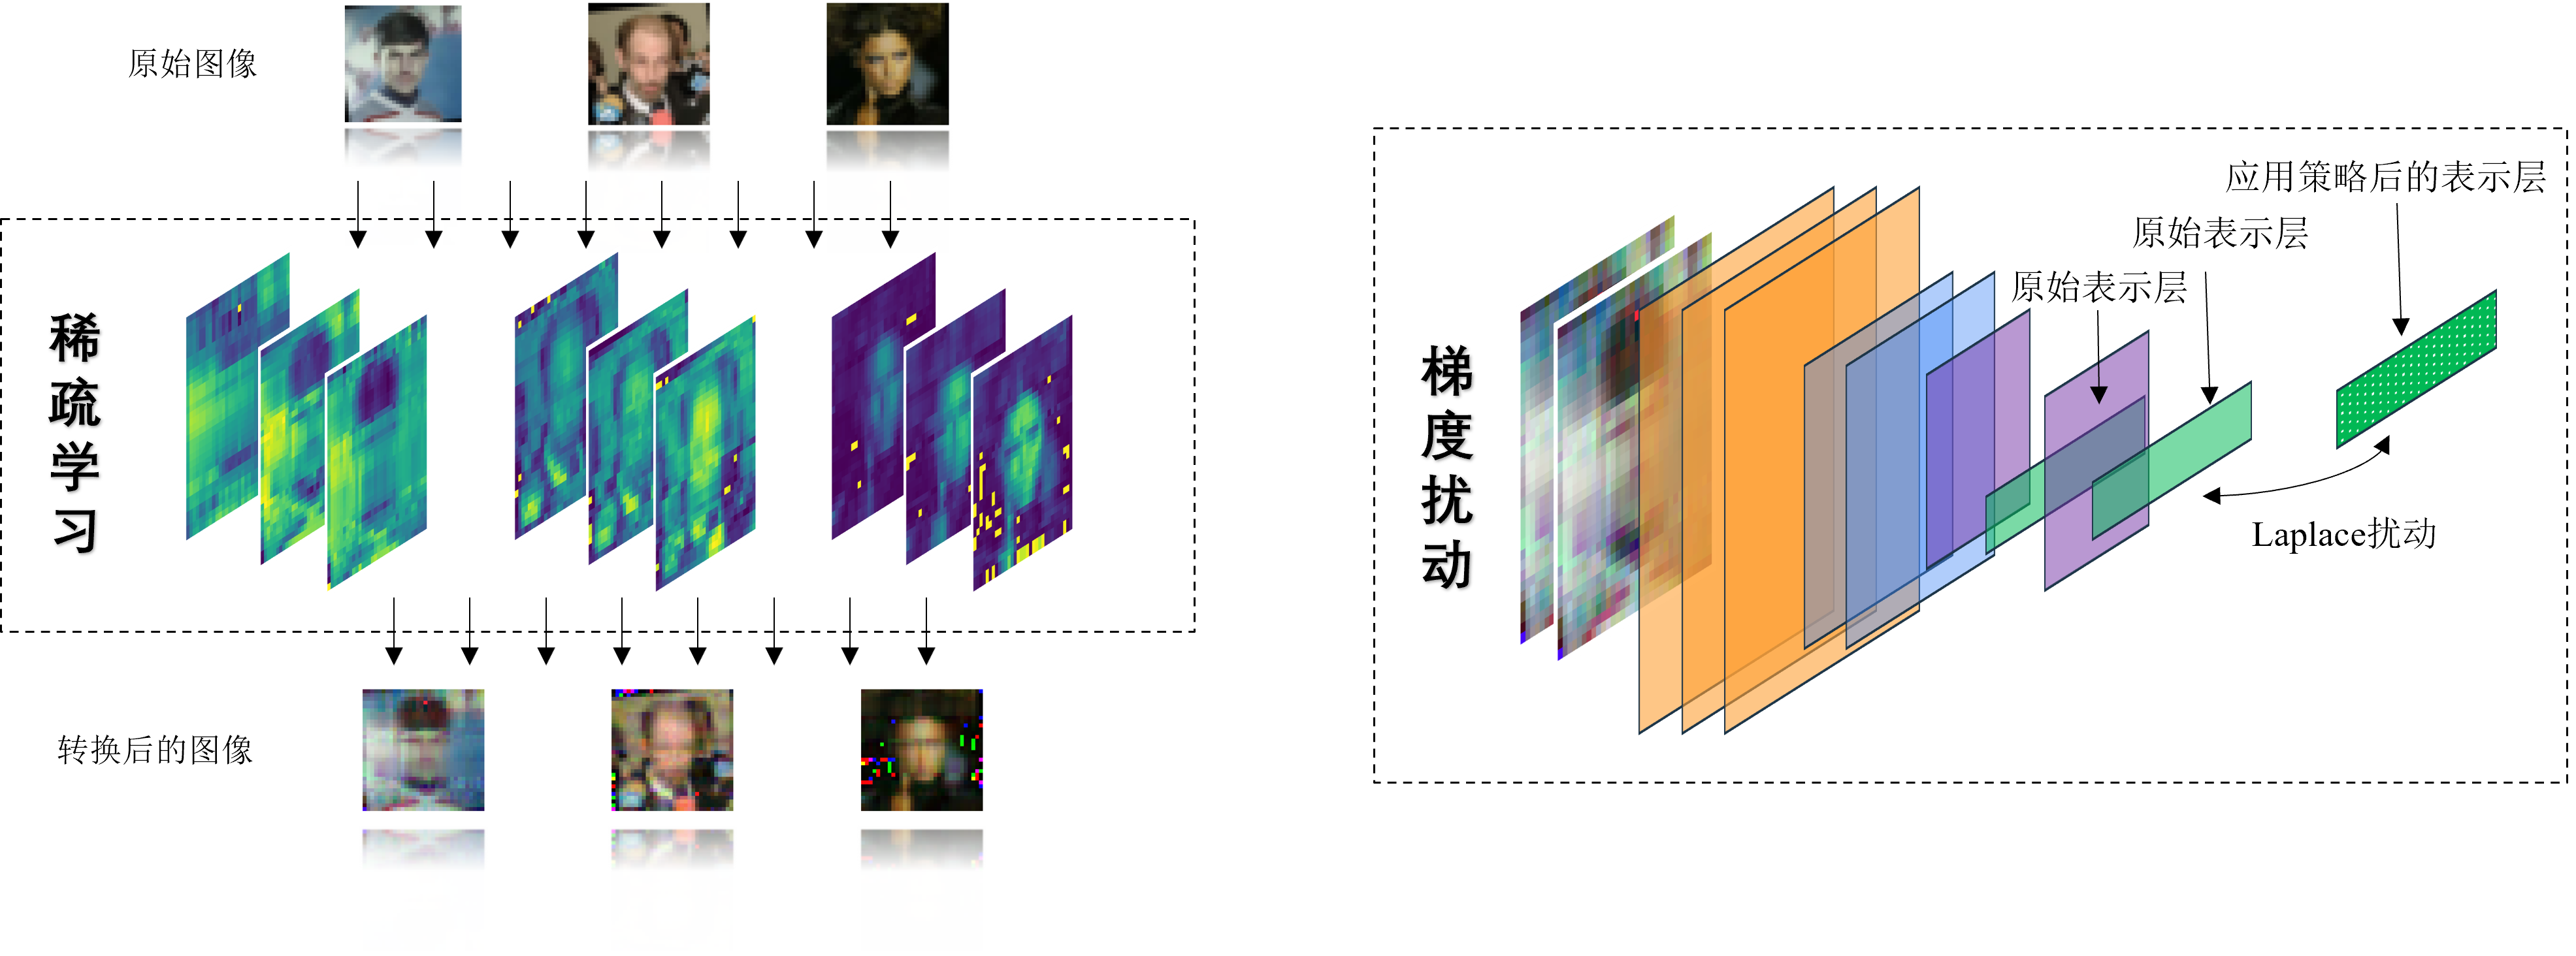
\includegraphics[scale=0.4]{figures/chapter4/chapter4.png}
    % \caption{FL-vgg16 Confusion Matrix}
    \caption{梯度泄露攻击的防御}
    \label{fig:Cluster the cars in the region}
\end{figure}

\subsection{梯度泄露攻击模型}

假设有一个神经网络$h_\theta:\mathbf{X}\to\mathbf{Y}$,使用参数$\theta$将输入空间$\mathbf{X}\subseteq\mathbb{R}^d$中的$x$映射到标签空间$\mathbf{Y}$中的$y$。假设输入$(x,y)$服从一个分布$\mathbf{D}$,则其边缘分布为$p(x)$。在本联邦学习系统中,有$n$个RSU,其各有一个损失函数$\mathbf{L}_1,\cdots,\mathbf{L}_n$,则要共同解决如下的优化问题:

\begin{equation}
\min_\theta\frac{1}{n}\sum_{i=1}^n\mathbb{E}{(x,y)\sim\mathbf{D}}\left[\mathbf{L}_i(h_\theta(x),y)\right]
\end{equation}

每一轮训练中,RSU$i$先在一组数据$(x_i,y_i)$上计算$\nabla_\theta \mathbf{L}_i(h_\theta(x_i),y_i)$,将其传给MEC。在MEC中使用一个梯度下降法,得到新的参数$\theta^{\prime}=\theta-\frac\alpha n\sum_{i=1}^n\nabla_\theta \mathbf{L}_i(h_\theta(x_i),y_i)$,$\alpha$是一个学习率。本节考虑一种情形,每个RSU上报的不是真实的梯度$\nabla_\theta \mathbf{L}_i(h_\theta(x_i),y_i)$,而是从分布$p(g|x)$中抽取的一个噪声梯度$g$,本节称之为防御机制。防御机制的目的是在梯度中加入足够的噪声,以掩盖用户的敏感信息,同时保留足够的信息量用于训练。因此,给定噪声梯度$g$,MEC将更新参数为$\theta^{\prime}=\theta-\frac\alpha n\sum_{i=1}^n g_i$。常见的防御例子是生成一个以截断的真实梯度为中心的噪声$p(g|x)$,比如在原始梯度上加上高斯(Gaussian)或拉普拉斯(Laplace)噪声,或者随机遮挡梯度的一些分量。$p(x)$和$p(g|x)$共同构成了一个联合分布$p(x,g)$。注意,没有防御的网络对应于分布$p(g|x)$,它只集中在$x$处的真实梯度上。

考虑一种场景,攻击者仅能观测到梯度 $g$,并试图从 $g$ 推断出产生它的输入 $x$。攻击者可以被视为一个函数 $f:\mathbb{R}^k\to \mathbf{X}$,其输入为梯度信息,输出一个重建的 $x$。设有一些 $(x,g)$ 的样本,它们服从联合分布 $p(x,g)$,则攻击者的重建 $f(g)$ 会导致一个损失 $\mathbf{L}'(x,f(g)):\mathbf{X}\times \mathbf{X} \to \mathbb{R}$。通常,采用一个二元损失,它仅在攻击者的重建和原始输入非常接近时为 $0$,否则为 $1$。若攻击者的目的是完全恢复输入 $x$,则损失可以定义为 $\mathbf{L}'(x,x^{\prime}):=\mathbf{O}_{x\neq x^{\prime}}$,其中 $\mathbf{O}$ 是指示函数。若攻击者的目的是找到输入 $x$ 在输入空间中的一个 $\delta$-邻域,则更适合的损失定义是 $\mathbf{L}'(x,x'):= \mathbf{O}_{d(x,x')>\delta}$,其中距离 $d$ 是 $\ell_{2}$ 距离。这种定义对于图像数据很有意义,因为 $\ell_{2}$ 距离能够反映人类对视觉相似度的感知,而且攻击者通常能够得到一个在视觉上或者在 $\ell_{2}$ 空间上都和原始图像很相似的重建。当 $\delta$ 趋近于 0 时,第二种损失定义就与第一种损失定义相同。基于此,可以定义攻击风险 $R(f)$ 为
\begin{equation}
\begin{aligned}
\frac{p_x(z)}{p_y(z)} &= \prod_{i=1}^{k} \frac{\exp\left(-\frac{e|f(x)_i - z_i|}{\Delta f}\right)}{\exp\left(-\frac{e|f(y)_i - z_i|}{\Delta f}\right)} \\
&= \prod_{i=1}^{k} \exp\left(\frac{e(|f(y)_i - z_i| - |f(x)_i - z_i|)}{\Delta f}\right) \\
& \leq \prod_{i=1}^{k} \exp\left(\frac{e(|f(x)_i - f(y)_i|)}{\Delta f}\right) \\
&= \exp\left(\frac{e \cdot ||f(x) - f(y)||_1 }{{\Delta f}}\right) \\
&\leq \exp(e)
\end{aligned}
\end{equation}


\subsection{基于稀疏学习的隐私保护策略}

本节的研究目标是找到一个转换函数$T$,使得每个原始输入$x$被转换为重构输入$\widehat{x}=T(x)$。因此,本节的研究目标可以分为以下两个方面:
\begin{itemize}
\item 目标 1:最小化重构输入和原始输入之间的相似度,以降低隐私泄漏风险。
\item 目标 2:最大化重构输入和原始输入表示的一致性,以保持FL的性能。
\end{itemize}

\subsubsection{隐私泄露得分$S_{pri}$}

针对目标1,本节引入隐私泄露得分$S_{pri}$,在\cite{Automatic_Transformation_Search_Against_Deep_Leakage_From_Gradients}的基础上加入攻击风险$R(f)$,用于衡量隐私信息泄露的程度,定义如下:
\begin{equation}
S_{pri}(T)=\frac{\gamma}{|\mathbb{R}|}\sum_{x\in \mathbb{R}} {Auc}(x,{\widehat{x}})+\beta{Var}_{T}+\delta R(f).
\end{equation}
为了简单起见,可以将这个得分近似为数值积分:
\begin{equation}
S_{pri}(T)\approx \frac{\gamma}{|\mathbb{R}|N}\sum_{x\in \mathbb{R}}\sum_{j=0}^{N-1}{CosSim}\bigg(x^{\prime}\bigg(\frac{j}{N}\bigg),{\widehat{x}}\bigg)+\beta{Var}_{T}+\delta R(f).
\end{equation}
其中$\gamma$,$\beta$,$\delta$分别是AUC面积(Area Under Curve)、方差和攻击风险的权重,$\gamma+\beta+\delta=1$,${x^{\prime}(i)}={(1-i)*x_{0}+i*\widehat{x}}$。

\begin{itemize}
    \item $ CosSim$:余弦相似度,用于衡量两个输入样本的梯度相似性,假设$x_{1},x_{2}$ 具有相同的标签$y$,当给定相同的模型参数$W$时:\begin{equation}  {CosSim}(x_{1}, x_{2}) = \frac{\langle \bigtriangledown W(x_{1}, y), \bigtriangledown W(x_{2}, y) \rangle }{|| \bigtriangledown W(x_{1}, y) || \cdot || \bigtriangledown W(x_{2}, y) ||}. \end{equation}$ {CosSim}$的范围是$[-1, 1]$,$-1$ 表示完全相反,$1$ 表示完全相同,$0$ 表示无关
    \item $ {Auc}$:$ {CosSim}$ 曲线下的面积,表示转换策略T在减少图像 $x$ 上的隐私泄露方面的有效性,一个好的转换策略会使得 $Auc$ 很小:\begin{equation}  {Auc}(x, {\widehat{x}}) = \int _{0}^{1}  {CosSim}(x^{\prime }(i), {\widehat{x}}) di. \label{eq:AUC}\end{equation}
    \item $ {Var}$:代表不同类别和样本之间$ CosSim$ 的方差,因为转换策略 $T$ 的 $ CosSim$ 值会随差异量大图像而变化,因此需要衡量转换策略$T$的整体效果,并保证数据集的隐私安全:\begin{equation}  {Var}= \frac{\Sigma _{x\in \mathbb{R}} ( {Auc}(x, {\widehat{x}}) - \bar{ {Auc}})^{2}}{|\mathbb{R}|}, \end{equation} $\bar{ {Auc}}$ 是 $\mathbb{R}$ 中所有样本的 AUC 得分的平均值。 $ {Var}_{T}$ 值越小,表示转换策略在抵抗重建攻击时,对不同类别的图像有一致的性能。
\end{itemize}

\subsubsection{准确度得分$S_{acc}$}

针对目标2,本节采用\cite{Neural_architecture_search_without_training}中的指标来量化策略对性能的影响。它根据经验评估了局部线性图与架构性能之间的相关性,并找出了能产生最佳性能的图。具体来说,准备一个随机初始化的模型$f$,以及由目标策略转换的一小批数据样本$\lbrace \widehat{x}_{n}\rbrace _{n=1}^{N}$。首先计算梯度雅可比矩阵,如下图所示:
\begin{equation} J = {\begin{pmatrix}\frac{\partial f}{\partial \widehat{x}_{1}}, & \frac{\partial f}{\partial \widehat{x}_{2}}, & \cdots & \frac{\partial f}{\partial \widehat{x}_{N}} \ \end{pmatrix}}^{\top }. \end{equation}
然后计算它的相关矩阵:
\begin{equation} \left(M_{J}\right)_{ i, j} = \frac{1}{N} \sum _{n=1}^{N}J_{i, n}, \ C_{J} = (J-M_{J})(J-M_{J})^{T}, \ \left(\Sigma _{J}\right)_{i, j} = \frac{\left(C_{J}\right)_{i, j}}{\sqrt{\left(C_{J}\right)_{i, i} \cdot \left(C_{J}\right)_{j, j} }}.  \end{equation}
令$\sigma _{J, 1} \leq \ldots \leq \sigma _{J, N}$ 为 $\Sigma_{J}$ 的 $N$个特征值。那么训练数据集中的准确率得分为
\begin{equation} S_{acc}(T)=\frac{1}{N}\sum _{i=0}^{N-1} {log(\sigma _{J,i} + \eta) + (\sigma _{J,i} + \eta)^{-1}},  \end{equation}

本节采用KSVD\cite{Deep_KSVD_Denoising}来实现转换函数$T$,用于其是一个低秩矩阵分解(Low-Rank Matrix Factorization)的问题,$\mathbf{X}$是一个给定的数据矩阵,$\boldsymbol{b}{j}$和$\boldsymbol{\omega}^{j}$是两组低秩矩阵,$k$是低秩的维度,$S_{pri}(T)$和$S_{acc}(T)$是两个优化目标函数,分别表示隐私保护(Privacy Protection)和准确性(Accuracy)的度量。一般来说,低秩矩阵分解的问题是非凸(Non-Convex)的,所以很难找到一个全局最优解。因此通常需要使用一些迭代算法(Iterative Algorithms),如梯度下降(Gradient Descent),交替最小二乘(Alternating Least Squares),或者随机梯度下降(Stochastic Gradient Descent),来逼近一个局部最优解。在这些算法中,$k$的取值会影响优化的结果和效率。一般来说,$k$越大,表示低秩矩阵的复杂度(Complexity)越高,能够更好地拟合数据矩阵$\mathbf{X}$,从而提高$S_{acc}(T)$的值。但是,$k$越大,也意味着低秩矩阵的稀疏性(Sparsity)越低,更容易泄露数据矩阵$\mathbf{X}$的信息,从而降低$S_{pri}(T)$的值。因此,$k$的取值需要在复杂度和稀疏性之间做一个平衡,以达到一个合理的折中方案。具体的$k$的取值,需要根据数据矩阵$\mathbf{X}$的特征,以及优化目标函数$S_{pri}(T)$和$S_{acc}(T)$的权重,算法流程如\ref{alg:Data sparsity algorithm}所示。

\begin{algorithm}[!th]
\caption{数据稀疏化}
\label{alg:Data sparsity algorithm}
\begin{algorithmic}[1]
    \REQUIRE 
        数据矩阵 $\mathbf{X}$, 低秩维度 $k$
    \ENSURE 
        转换函数 $T$, 重构输入 $\widehat{\mathbf{X}}$
    \STATE 初始化 $\widehat{\mathbf{X}} = T(\mathbf{X})$
    \STATE 初始化 $S_{pri}(T)$ 和 $S_{acc}(T)$
    \REPEAT
    % \STATE \textbf{functinon} Data\_sparsity\_algorithm()
        \FOR{each $j \in {1, \dots, k}$}
        \STATE Compute $S_{pri}(T')=\min(S_{pri}(T),\gamma{Auc}+\beta{Var}+\delta R(f))$
        \STATE Compute $S_{acc}(T')=\max(S_{acc}(T),\frac{1}{N}\sum _{i=0}^{N-1} {log(\sigma _{J,i} + \eta) + (\sigma _{J,i} + \eta)^{-1}})$
        \STATE Update $\widehat{\mathbf{X}}_j = T_j(\mathbf{X}_j)$
        \ENDFOR
        \STATE Update $\widehat{\mathbf{X}} = [\widehat{\mathbf{X}}_1, \dots, \widehat{\mathbf{X}}_k]$
    \UNTIL{收敛或达到最大迭代次数}
    \RETURN $T$
    % \STATE \textbf{end function}
    \end{algorithmic}
\end{algorithm}

\subsection{基于DP-SGD的梯度扰动策略}

联邦学习(FL)是一种分布式的机器学习方法,它允许多个参与者在本地使用自己的数据训练模型,然后将模型参数或更新信息发送给中心服务器,从而保护了用户数据的隐私。但是,这种方法仍然存在隐私泄漏的风险,因为数据表示层的信息可能会通过模型参数或更新信息泄露出去\cite{Soteria}。例如,恶意的参与者可以通过梯度信息,利用一些逆向工程的技术,重构出其他参与者的训练数据。为了解决这个问题,Gao等人\cite{Automatic_Transformation_Search_Against_Deep_Leakage_From_Gradients}提出了一种基于图像转换技术的隐私保护方案,它可以在保证模型性能的同时,有效地减少梯度信息的泄漏。然而,这种方案的一个缺点是,它会将一些扰动后的梯度设置为0,导致模型训练时的精度损失。因此,本节提出了一种改进的方案,将DP-SGD方案与梯度扰动方案结合,以实现更高效和更安全的隐私保护。

令$r$和$r^{\prime}$分别表示被防御层的干净数据表示和扰动数据表示。定义$x$和$x^{\prime}$为原始输入和通过扰动数据表示重构的输入。该方案的目标是在满足两个条件的情况下,最大化$x$和$x^{\prime}$之间的距离,以$L_2$范数衡量。这两个条件分别是:
\begin{itemize}
\item 目标1:$x$和$x^{\prime}$之间的距离应该尽可能大,以增加重构的难度和误差;
\item 目标2:$r$和$r^{\prime}$之间的距离应该有界,以保证扰动后的数据表示仍然能够保持模型的性能。
\end{itemize}
为了实现这个目标,该方案首先假设存在一个特征提取器$f:x\rightarrow r$,它可以将原始输入映射到数据表示层,以及它的逆函数$f^{-1}$,它可以将数据表示层映射回原始输入。进一步假设$f^{-1}$在$r$上是可微的,并且对于任意满足$||r-r'||_0\leq\epsilon$的$r'$,都有$f^{-1}(r')$存在。此外,根据链式法则,有$\nabla_{r}f^{-1}=(\nabla_{x}f)^{-1}$。基于这些假设,目标函数可以简化为:
\begin{equation}\begin{aligned}
&r^{\prime}\approx\arg\max_{r^{\prime}}\left\|\nabla_rf^{-1}\cdot(r-r^{\prime})\right\|_2,\mathrm{~s.t.~}\left\|r-r^{\prime}\right\|_0\leq\varepsilon\\
&=\arg\max_{r^{\prime}}\left\|\left(\nabla_xf\right)^{-1}\cdot\left(r-r^{\prime}\right)\right\|_2,\mathrm{~s.t.~}\left\|r-r^{\prime}\right\|_0\leq\varepsilon,
\end{aligned}\end{equation}
因此,该解决方案是在集合$\{||r_i(\nabla_xf(r_i))^{-1}||_2\}$中找到$\epsilon$个最大的元素,然后将它们对应的$r_i$作为扰动数据表示。这样,不仅可以提高重构的难度,还可以降低通信的开销,因为只需要传输非零的扰动数据表示。本文将其扩展到模型所有的表示层中,避免梯度冻结带来的防御策略失效现象,详细内容如算法\ref{alg:ImprovedDP-SGD}所示。

\begin{algorithm}[!htb]
\caption{改进版梯度扰动}
\label{alg:ImprovedDP-SGD}
\begin{algorithmic}[1]
\REQUIRE 数据矩阵 $\mathbf{X}$,损失函数$\nabla_\theta \mathbf{L}_i(h_\theta(\mathbf{X}),\mathbf{Y}))$,第$i$次迭代所需的学习率$\eta_i$, 噪声规模$\sigma$,组大小$\mathcal{G}$, 防御层之前的特征提取器$f: \mathbb{R}^{M \times N} \to \mathbb{R}^L$,干净的数据表示$r \in \mathbb{R}^L$,扰动边界$\epsilon$
\STATE 初始化 $\theta_{0}$
\FOR{each $i\in 1,\cdots,N$}
\STATE  在抽样概率 $q=\frac{\mathcal{G}}{n}$ 下随机抽样 $\mathcal{G}_i$。
\FOR{each $j\in \mathcal{G}_i$}
    \STATE \quad Compute $\widehat{\mathbf{x}}_j = T(x_j)$
    \STATE \quad Compute $g_i(x_j)=\nabla_\theta \mathbf{L}_j(h_\theta(\widehat{\mathbf{x}}_j),y_j)$
\ENDFOR

\FOR{each $j \in \text{Size}(g_i)$}
    \STATE \quad  提取$g_i$中的表示层,赋值索引为$k$
     \STATE \quad Compute $\mathbf{f}_i(r_k)=||r_k(\nabla_{\widehat{\mathbf{x}}_j}f(r_k)^{-1}||_{2}$
     \STATE \quad $\text{Find}\ \mathbf{f}_i$中$\epsilon$个最大元素的索引集合$S$
     \STATE \quad Set $r'_m=\zeta_{Lap},\text{if} \  m \in S$。
\ENDFOR
\STATE  $\theta_{t+1}=\theta_i-\eta_i g_i$
\ENDFOR
    % \STATE \textbf{end function}
\end{algorithmic}
\end{algorithm}

\section{基于稀疏学习和梯度扰动的梯度泄露防护实验}
\subsection{实验设置和实现细节}

% 数据集和模型。在不损失通用性的前提下,在两个数据集(CIFAR10\cite{cifar10}、Fashion MNIST(F-MNIST)\cite{Fashion-MNIST})和常规 LeNet 模型上验证提出方法的有效性。为了证明先进性,在三个数据集(LFW (Labeled Faces in the Wild)数据集\cite{LFW}、MNIST数据集、CIFAR-100数据集\cite{cifar10})和LeNet模型上,同其他方法方法进行横向对比。所有的数据集都按照8:2进行训练集和测试集的划分。

% 训练配置。实验在一台Ubuntu服务器上,其配置为Intel(R) Core(TM) i9-10980XE CPU @ 3.00GHz,GPU 型号是 TITAN RTX,这是一款高端的专业级显卡,它拥有 4608 个 CUDA 核心,24 GB 的 GDDR6 显存,672 GB/s 的显存带宽,16.3 TFLOPS 的单精度浮点性能,以及 130 TFLOPS 的张量核心性能。 采用带有动量、权重衰减和学习衰减技术的 SGD 优化器来保证全局模型的收敛性。具体而言,动量为 0.9、权重衰减为 $2\cdot 10^{-3}$ 的 SGD 来优化深度神经网络,批次大小都为200,对于梯度泄露防御以测试模型对隐私保护的防御能力是,训练历元设置为300轮,在进行图像分类以测试模型分类能力是训练50轮。

% 攻击实现。本章在实验中评估了两种攻击,以“优化器+距离测量”的格式命名。这些技术涵盖不同的优化器和距离度量:(1)采用LBFGS和L2范数进行优化的DLG(LBFGS+L2)\cite{DLG};(2)IG(adam+余弦)\cite{Inverting_Gradients},采用adam和余弦距离进行优化;

数据集和模型。本文提出了一种基于梯度泄露的隐私保护方法,为了验证其有效性和先进性,在两类数据集和一个经典的深度神经网络模型上进行了实验。这两类数据集分别是:(1)自然图像数据集,包括 CIFAR10\cite{cifar10}、CIFAR100\cite{cifar10} 和 Fashion MNIST(F-MNIST)\cite{Fashion-MNIST},它们包含了不同的图像类别和复杂度,可以用来测试模型的分类能力和鲁棒性;(2)人脸图像数据集 LFW (Labeled Faces in the Wild)数据集\cite{LFW},它包含了多个人脸的不同角度和表情,可以用来测试模型的识别能力和对抗性。选择 LeNet 作为深度神经网络模型,它是一个简单而有效的卷积神经网络,广泛应用于图像处理领域。将本文的方法与其他几种方法在这些数据集和模型上进行了横向对比,以展示所提出方法的优势和局限。为了保证实验的公平性,将所有的数据集都按照 8:2 的比例划分为训练集和测试集。

训练配置。实验环境是一台配置优良的 Ubuntu 服务器,其具体参数如下:处理器为 Intel(R) Core(TM) i9-10980XE CPU @ 3.00GHz,具有 18 个物理核心和 36 个逻辑核心,显卡为 TITAN RTX,拥有 4608 个 CUDA 核心,24 GB 的 GDDR6 显存,内存为 128 GB。本文使用 SGD 优化器来训练深度神经网络,这是一种常用的优化算法,可以有效地降低模型的损失函数。本文为 SGD 优化器设置了一些技术参数,以提高模型的收敛速度和稳定性,具体如下:动量为 0.9,可以加速模型的收敛方向和避免陷入局部最优;权重衰减为 $2\cdot 10^{-3}$,可以防止模型的过拟合和正则化模型的复杂度;学习率为 0.01,并且每 50 轮衰减为原来的 0.1,可以根据模型的训练进度动态地调整学习率的大小,以平衡模型的收敛速度和精度。本文将批次大小设置为 200,这意味着每次训练从训练集中随机抽取 200 个样本作为输入,以减少模型的内存占用和计算时间。本文根据不同的实验目的,设置了不同的训练轮数,具体如下:对于梯度泄露防御的实验,设置了 300 轮,以测试模型对隐私保护的防御能力;对于图像分类的实验,设置了 50 轮,以测试模型的分类能力。

攻击实现。为了评估本文提出方法的隐私保护效果,在实验中实现了两种常见的梯度泄露攻击,它们都是基于优化器和距离测量的方法,可以从模型的梯度中重构出原始的输入数据。这两种攻击分别是:(1)DLG(LBFGS+$L_2$)\cite{DLG},使用了 LBFGS 作为优化器利用历史信息来更新梯度方向和步长,从而加速优化过程;使用了 $L_2$ 范数作为距离测量,用于衡量两个向量之间的相似度,从而评估重构的质量;(2)IG(adam+余弦)\cite{Inverting_Gradients},使用了 Adam 作为优化器,根据梯度的变化情况动态地调整学习率和动量,从而适应不同的优化场景;使用了余弦距离作为距离测量,衡量两个向量之间的方向相似度,从而忽略向量的长度差异。本文将这两种攻击分别应用于所提出方法和其他几种方法,以比较它们的隐私保护性能和重构效果。

\subsection{策略的有效性评估}

本节提出的防御方法可以达到令人满意的变换策略。图\ref{fig:CIFAR10 with ours in DLG}展示了在 CIFAR10\cite{cifar10}和Fashion MNIST(F-MNIST)\cite{Fashion-MNIST}数据集的 DL 攻击 \cite{DLG} 下,使用和不使用策略重建图像的直观对比。观察到,在没有任何转换的情况下,攻击者可以非常高的保真度恢复图像(第 3 行 和 第 6 行)。相反,训练样本经过转换后(第 2 行和 第 5 行),攻击者几乎无法从恢复的图像中获得任何有意义的信息(第 4 行)。本节在其他数据集上(图\ref{fig:Defense strategy comparison experiment})也得到了类似的结果。

\begin{figure}[htb]
\centering
    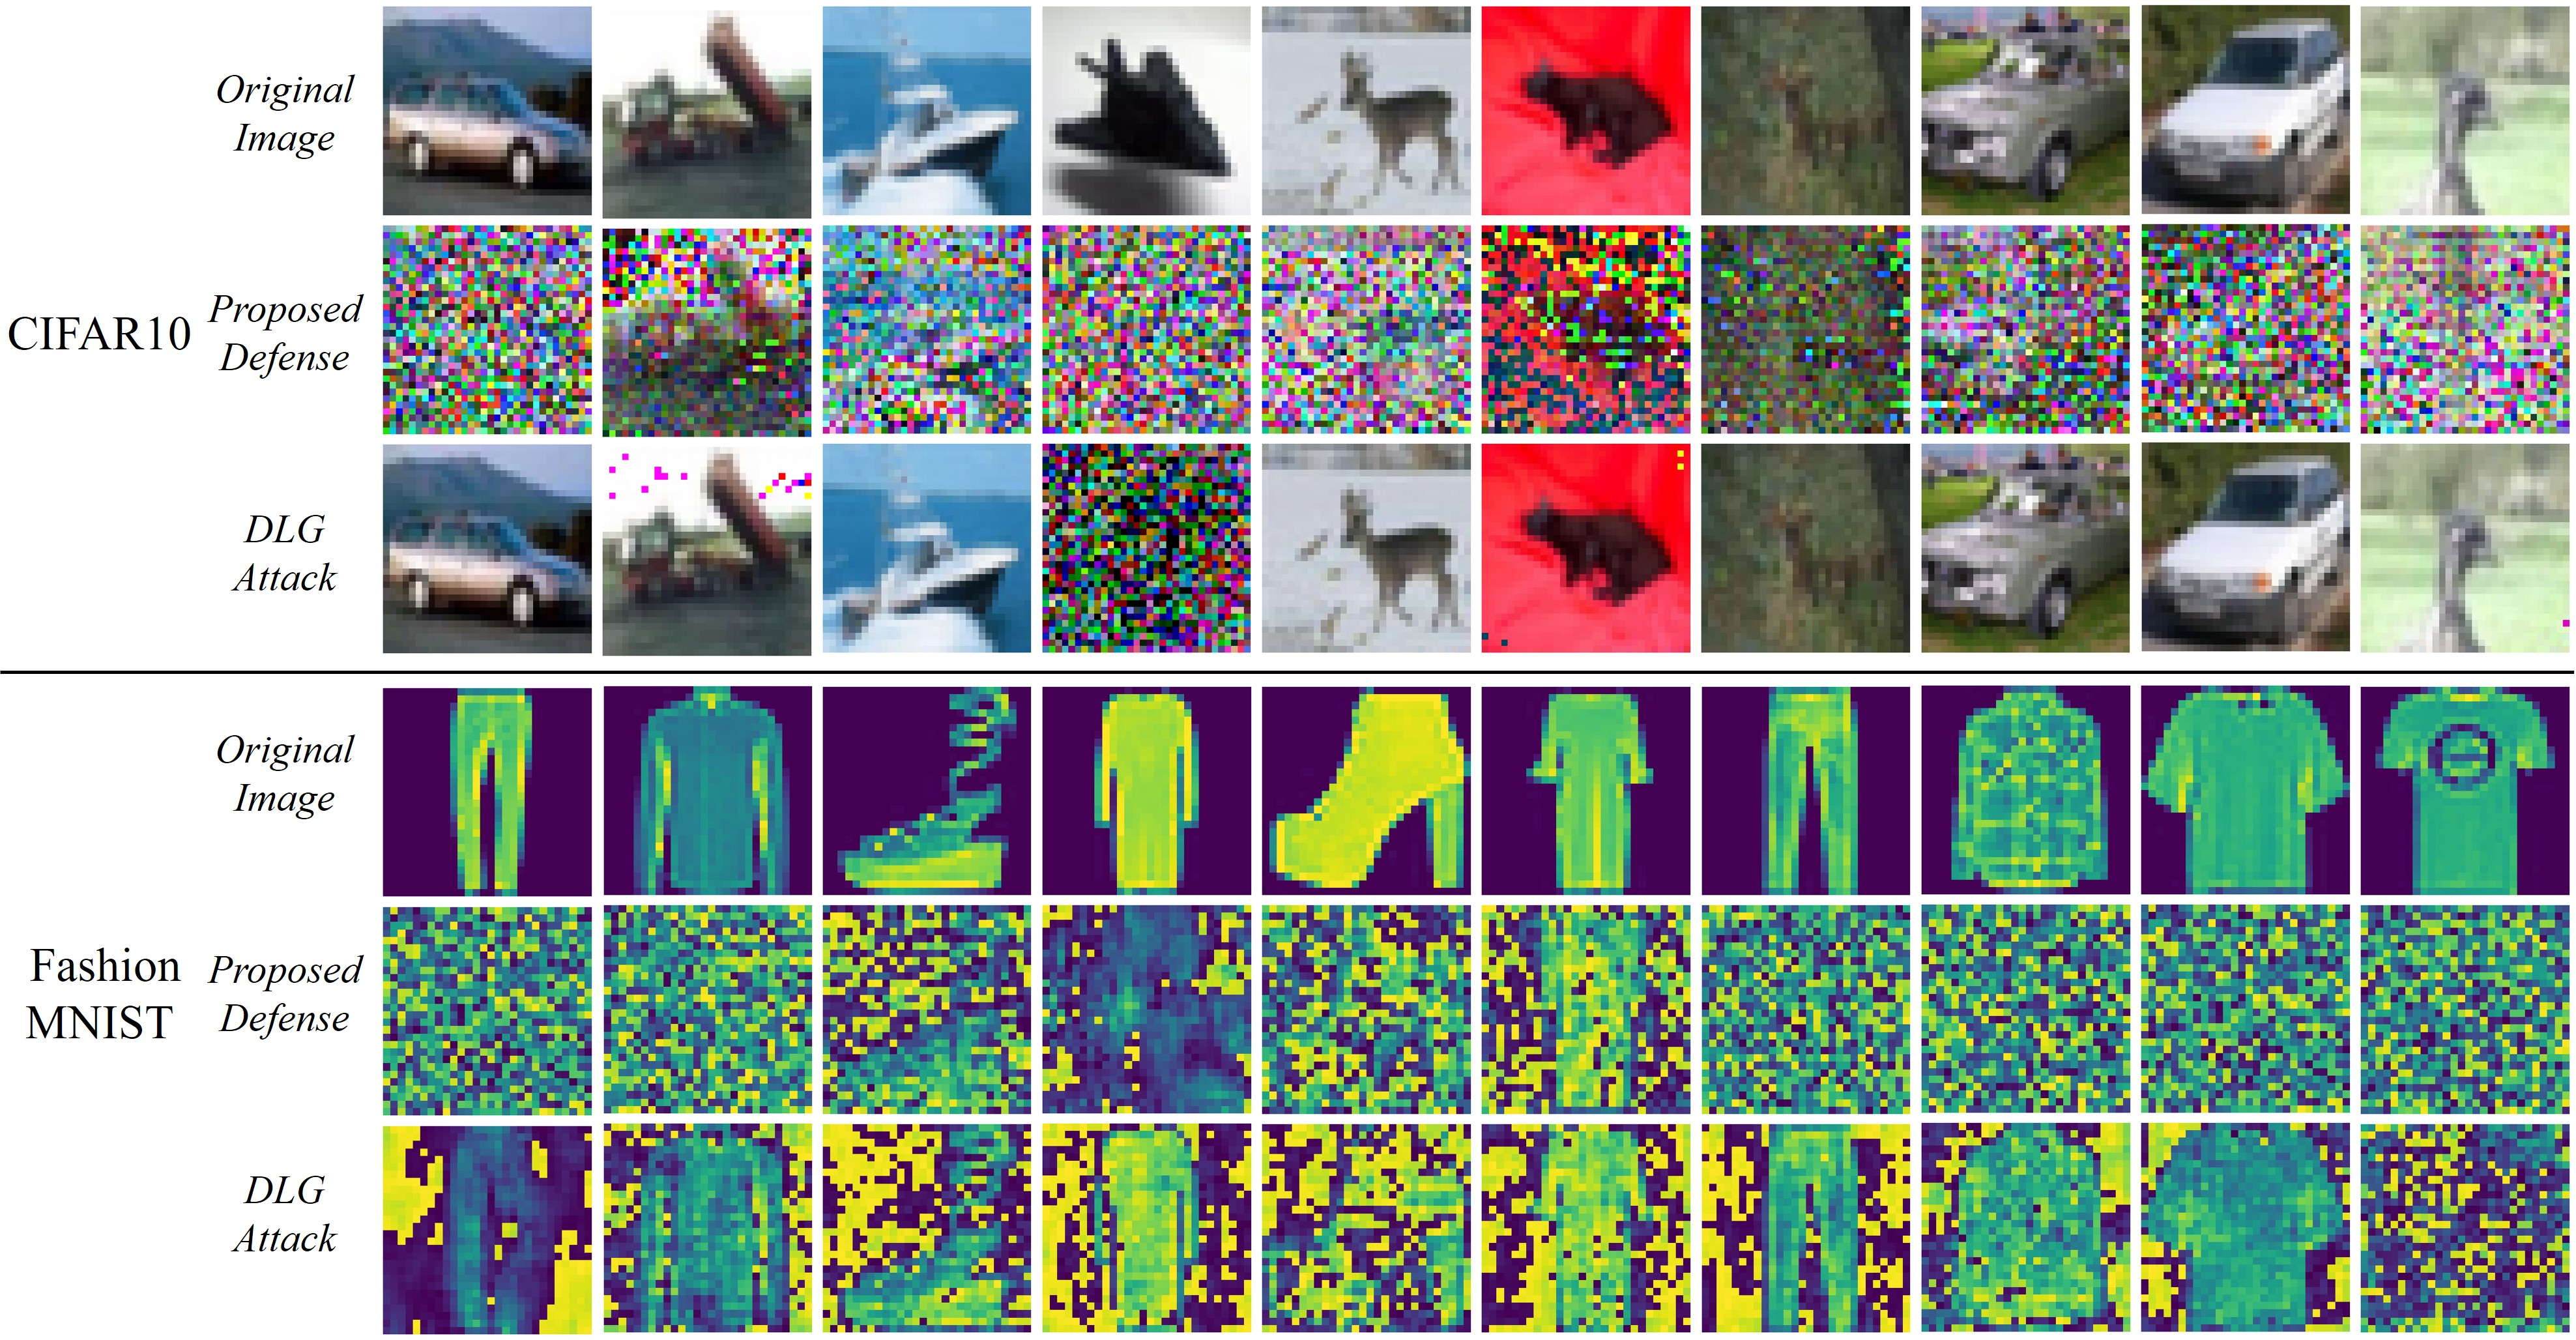
\includegraphics[scale=0.5]{figures/chapter4/Comparative experiment of strategy effectiveness.jpg}
    % \caption{FL-vgg16 Confusion Matrix}
    \caption{在CIFAR10和MNIST数据集上使用和未使用本节的防御方法进行重构攻击的可视化结果。第 1 行:原始样本,第 2 行:应用本节方法的样本,第 3 行:未使用任何防御。}
    \label{fig:CIFAR10 with ours in DLG}
\end{figure}

与其他防御方法的比较。为了评估本节提出的防御方法在不同数据集上的效果,本文将其与其他几种防御方法进行了对比,包括差分隐私(DP-Laplace 和 DP-Gaussian)、剪枝技术(GC)和 Sotria。本文使用了三个指标来衡量防御方法的性能,分别是 PSNR(峰值信噪比)、IIP-pixel(像素级逆向攻击指数)和 SSIM(结构相似性)。其中,PSNR 和 SSIM 越低,表示重构图像的质量越差,防御效果越好;IIP-pixel 越低,表示重构图像与原始图像的相似度越低,防御效果越好。图 \ref{fig:Defense strategy comparison experiment} 和表 \ref{tab:Defense strategy comparison experiment} 展示了在 LFW、MNIST 和 CIFAR-100 三个数据集上的对比结果。

\begin{figure}[htb]
    \centering
    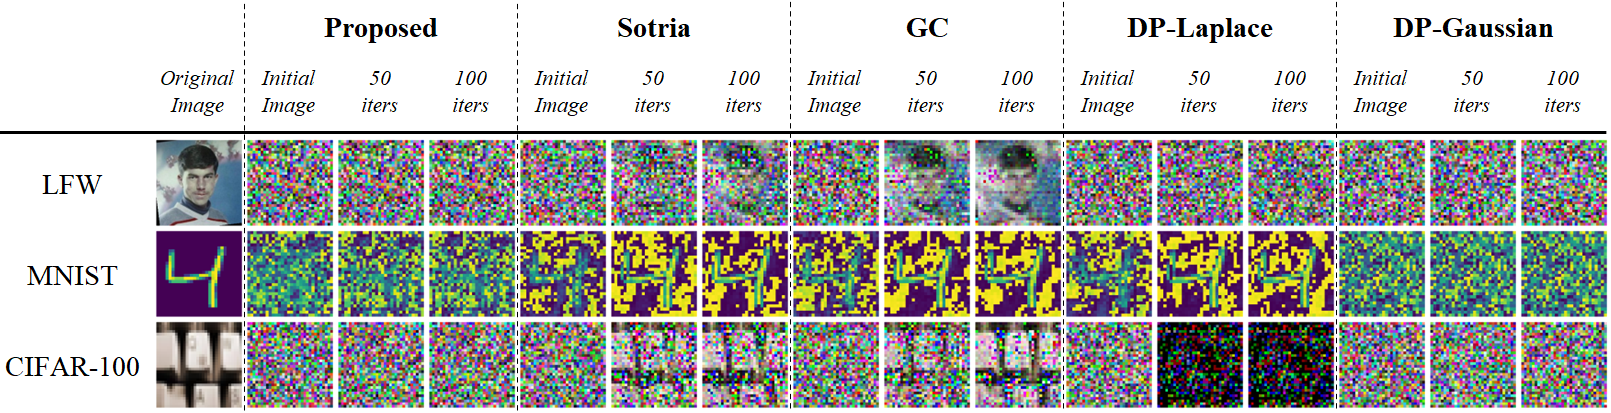
\includegraphics[width=1.0 \textwidth]{figures/chapter4/contrast experiment.png}
    \caption{本节的防御方法与其他防御方法在多个数据集上的对比结果}
     \label{fig:Defense strategy comparison experiment}
\end{figure}

从图 \ref{fig:Defense strategy comparison experiment} 中可以看出,本节的防御方法在所有数据集上都能显著降低 PSNR 和 SSIM 值,说明重构图像的质量很差,难以识别出原始图像的内容。从表 \ref{tab:Defense strategy comparison experiment} 中可以看出,本节的防御方法在所有数据集上都能达到最低的 IIP-pixel 值,说明重构图像与原始图像的相似度很低,难以进行像素级的逆向攻击。这些结果表明,本节的防御方法能有效地抵抗梯度泄露攻击,保护数据的隐私。相比之下,其他防御方法的效果都不理想。差分隐私方法虽然能降低 PSNR 和 SSIM 值,但是 IIP-pixel 值却很高,说明重构图像仍然保留了原始图像的一些特征,容易被逆向攻击。剪枝技术的效果更差,它几乎不能降低任何指标的值,说明重构图像的质量很高,与原始图像非常相似,没有达到防御的目的。Sotria 方法的效果也不稳定,它在某些数据集上能降低 PSNR 和 SSIM 值,但是在其他数据集上却反而提高了这些值,说明重构图像的质量与原始图像的复杂度有关,防御效果不一致。

\begin{table}[t]
\scriptsize
    \centering
    \begin{tabular}{lccccc}\hline
        &  & \textbf{LFW} & \textbf{MNIST} & \textbf{CIFAR-100} \\ \hline
        \multirow{3}{*}{\makecell{Proposed}}
        & PSNR & \textbf{10.620} & 10.014 & 8.935 \\
        & IIP-pixel & \textbf{0.318} &  \textbf{0.475} & \textbf{0.374} \\
        & SSIM & \textbf{0.431} &	\textbf{0.545} &	0.446 \\  \hline

        \multirow{3}{*}{\makecell{Sotria}}
        & PSNR &12.957 &	10.141 &	11.176  \\
        & IIP-pixel &0.343 &	0.552 &	0.491  \\
        & SSIM & 0.480 &	0.679 &	0.579  \\ \hline
        
        \multirow{3}{*}{\makecell{GC}}
        & PSNR & 18.609 &	9.460 &	12.424 \\
        & IIP-pixel & 0.369 &	0.513 &	0.523 \\
        & SSIM & 0.598 &	0.661 &	0.660 \\ \hline

        \multirow{3}{*}{\makecell{DP-Laplace}}
        & PSNR & 10.809 &	\textbf{9.413} &	\textbf{6.964} \\
        & IIP-pixel & 0.320 &	0.510 &	0.466 & \\
        & SSIM & 0.434 & 0.651 & \textbf{0.360}  \\ \hline
        
        \multirow{3}{*}{\makecell{DP-Gaussian}}
        & PSNR & 10.577 &	10.294 &	9.001 \\
        & IIP-pixel & 0.320 &	0.477 &	0.381 \\
        & SSIM & 0.432 &	0.536 &	0.448 \\ \hline
    \end{tabular}%
    \caption{\textmd{本节的防御方法与其他防御方法在多个数据集上的数值对比结果(取最后一轮结果)}}
    \label{tab:Defense strategy comparison experiment}
\end{table}

%此外,Sotria 方法还会导致模型的准确性明显下降,这是本节的防御方法所不具备的。综上所述,本节的防御方法在保持高模型准确性的同时,还能显著改善重构图像的质量,是一种有效的防御方法。

% \subsection{对模型性能影响}


\section{本章小结}

本节针对深度学习模型的梯度泄露攻击进行了详细的分析和研究,提出了一个基于稀疏学习和梯度扰动的梯度泄露防护的隐私保护策略。该策略主要包括两个方面:一是在模型训练的时候,利用基于稀疏矩阵的数据提取方案,将原始数据转化为稀疏化后的数据,从而降低数据的敏感性和可识别性;二是在模型训练过程中,对模型的所有表示层应用差分隐私与梯度扰动的隐私保护策略,通过在梯度上添加合适的噪声,防止梯度泄露攻击者利用梯度信息恢复出原始数据或模型参数。本节通过实验验证了该策略的有效性和模型性能影响,实验结果表明,本节提出的方案在隐私保护性和模型影响性方面都优于现有的流行方案,能够有效地抵御梯度泄露攻击,同时保持模型的高精度和泛化能力。
